%%%%%%%%%%%%%%%%%%%%%%%%%%%%%%%%%%%%%%%%%%%%%%%%%%%%%%%%%%%%%%%%%%%%%%
% How to use writeLaTeX: 
%
% You edit the source code here on the left, and the preview on the
% right shows you the result within a few seconds.
%
% Bookmark this page and share the URL with your co-authors. They can
% edit at the same time!
%
% You can upload figures, bibliographies, custom classes and
% styles using the files menu.
%
%%%%%%%%%%%%%%%%%%%%%%%%%%%%%%%%%%%%%%%%%%%%%%%%%%%%%%%%%%%%%%%%%%%%%%

\documentclass[12pt]{article}
\usepackage{subcaption}
\usepackage{sbc-template}
\usepackage{float}

\usepackage{graphicx,url}

\usepackage{graphicx}

\usepackage[brazil]{babel}   
\usepackage[utf8]{inputenc}  
\usepackage{geometry}
\usepackage{float}
\usepackage{sbc-template}
\usepackage{bera}% optional: just to have a nice mono-spaced font
\usepackage{listings}
\usepackage{xcolor}
\usepackage{booktabs}
\usepackage{verbatim}
\usepackage{amsmath}
     
\sloppy

\title{Avaliação de estratégias para escolha do elemento pivô no algoritmo Quicksort}

\author{Jaime Antonio Daniel Filho\inst{1}}
\address{Curso de Ciência da Computação, Universidade Federal de Santa Maria
  (UFSM)\\
  \email{jafilho@inf.ufsm.br}
}
\begin{document} 

\maketitle

\section{Introdução}

O Quicksort é um algoritmo de ordenação baseado na estratégia de divisão e conquista, introduzido por Tony Hoare na década de 1960, e é amplamente utilizado pela sua eficiência prática em uma grande variedade de cenários. A abordagem de divisão e conquista do Quicksort funciona dividindo o conjunto de dados em duas partes ao escolher um elemento específico, conhecido como pivô. Durante cada iteração, os elementos menores que o pivô são movidos para a esquerda, enquanto os elementos maiores são movidos para a direita. Essa partição continua de maneira recursiva até que todas as divisões sejam suficientemente pequenas para que o conjunto esteja ordenado.

A complexidade de tempo do Quicksort varia de acordo com a disposição inicial dos dados e a escolha do pivô. No melhor caso, quando a divisão dos dados é balanceada, a complexidade é $O(n \log{n})$. No caso médio, ainda que as divisões não sejam perfeitamente balanceadas, a complexidade esperada também é $O(n \log{n)}$. No entanto, no pior caso, o Quicksort se degenera para uma complexidade quadrática $O(n^2)$, o que ocorre quando o pivô não é bem escolhido, resultando em partições desbalanceadas. Este trabalho se propõe a analisar o número de comparações realizadas no Quicksort ao escolher diferentes posições do pivô (primeiro, último e meio) em três tipos de conjuntos de dados: crescentes, decrescentes e aleatórios.

Neste estudo, a partição foi implementada utilizando o método de Hoare, onde o elemento escolhido como pivô é trocado com o primeiro elemento do vetor antes de iniciar o processo de ordenação. Esse método é amplamente conhecido por sua simplicidade e, quando combinado com uma boa estratégia de escolha do pivô, pode minimizar o número de comparações e a profundidade de recursão, tornando o algoritmo mais eficiente.

\section{Metodologia}

Para quantificar o impacto da escolha do pivô, testamos conjuntos de dados com quantidades variáveis de elementos, de 0 a 100.000, aumentando em intervalos de 1.000 elementos. No cenário com dados aleatórios, realizamos 100 testes para cada escolha de pivô e calculamos a média do número de comparações realizadas. Os gráficos a seguir ilustram o número de comparações médio para cada escolha de pivô em relação aos tipos de dados analisados.

\section{Resultados}

Na Figura \ref{fig:asc}, vemos o comportamento do Quicksort com dados ordenados de forma crescente. Com a escolha do primeiro ou último elemento como pivô, observamos que o número de comparações aumenta de forma quadrática com o aumento do tamanho do conjunto de dados, refletindo o pior caso do algoritmo. Esse comportamento ocorre porque a ordenação crescente faz com que o Quicksort parta repetidamente de subvetores muito desbalanceados, pois o pivô acaba ficando no extremo das partições. No entanto, ao escolher o elemento do meio como pivô, o desempenho melhora significativamente, resultando em um número de comparações mais baixo e próximo de $O(n \log{n)}$, uma vez que a divisão dos dados tende a ser mais balanceada.

\begin{figure}[H]
\centering
\caption{Número de comparações com dados crescentes}
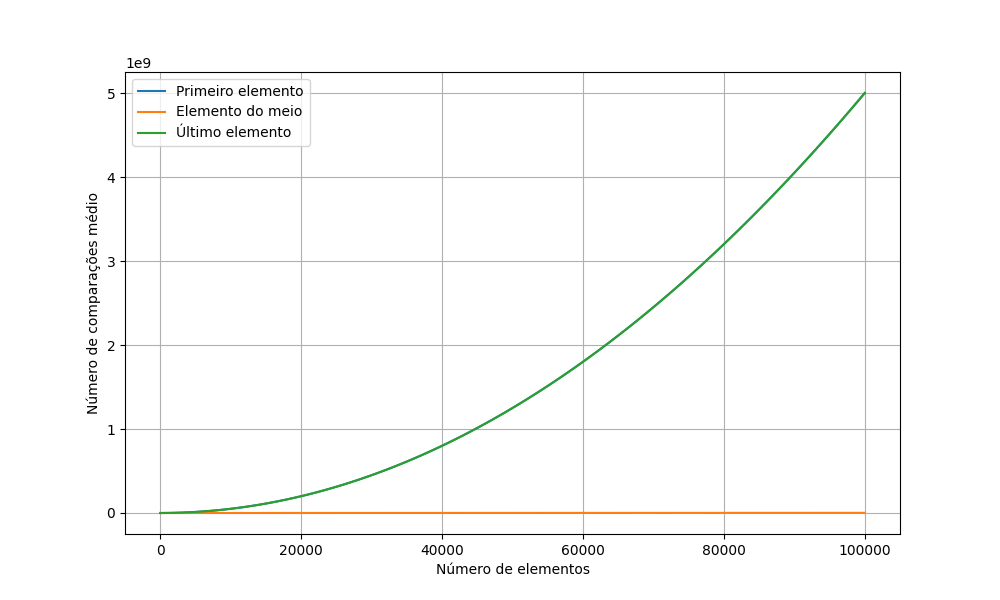
\includegraphics[width=0.85\textwidth]{ascending.png}
\label{fig:asc}
\end{figure}

A Figura \ref{fig:desc} ilustra o número de comparações para conjuntos ordenados de forma decrescente, e os resultados foram muito semelhantes aos obtidos com dados crescentes. Novamente, ao utilizar o primeiro ou último elemento como pivô, o algoritmo apresentou uma complexidade quadrática devido às partições desbalanceadas. Esses resultados destacam que dados previamente ordenados em qualquer ordem representam o pior caso para o Quicksort, uma vez que o processo de divisão se torna altamente desbalanceado. Escolher o elemento central como pivô, no entanto, leva a uma divisão mais equilibrada dos dados, proporcionando uma redução no número de comparações.

\begin{figure}[H]
\centering
\caption{Número de comparações com dados decrescentes}
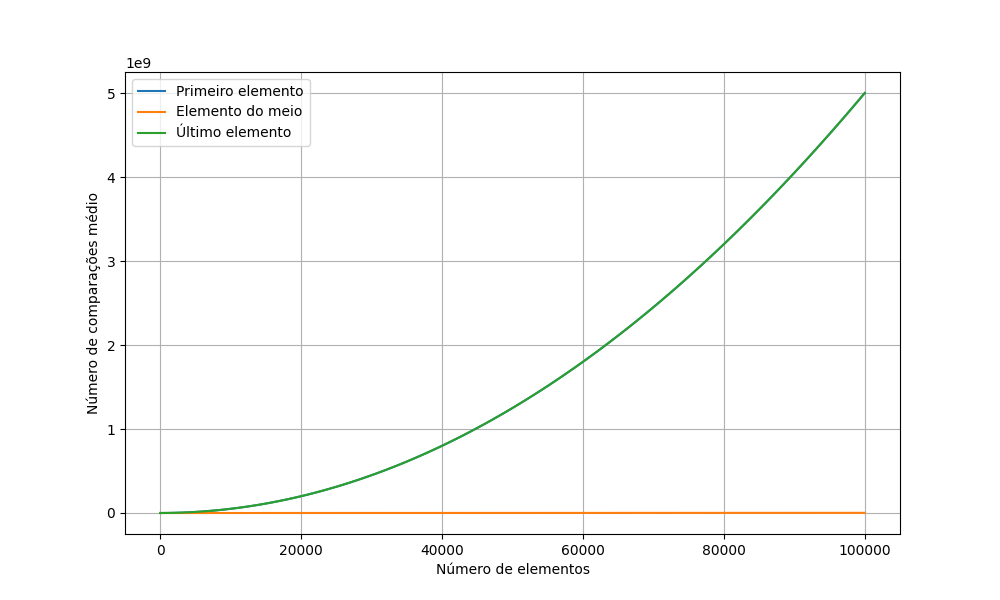
\includegraphics[width=0.85\textwidth]{descending.png}
\label{fig:desc}
\end{figure}

A Figura \ref{fig:rand} mostra o desempenho do Quicksort com dados aleatórios. Nesse cenário, todas as escolhas de pivô apresentaram desempenho semelhante, o que reflete a distribuição aleatória dos dados. No entanto, ao analisar a média das comparações, a escolha do elemento central como pivô ainda teve um leve benefício em relação às outras duas abordagens. Esse comportamento é consistente com a expectativa de que o elemento central minimiza a probabilidade de partições desbalanceadas e, portanto, reduz ligeiramente o número de comparações.

\begin{figure}[H]
\centering
\caption{Número de comparações com dados aleatórios}
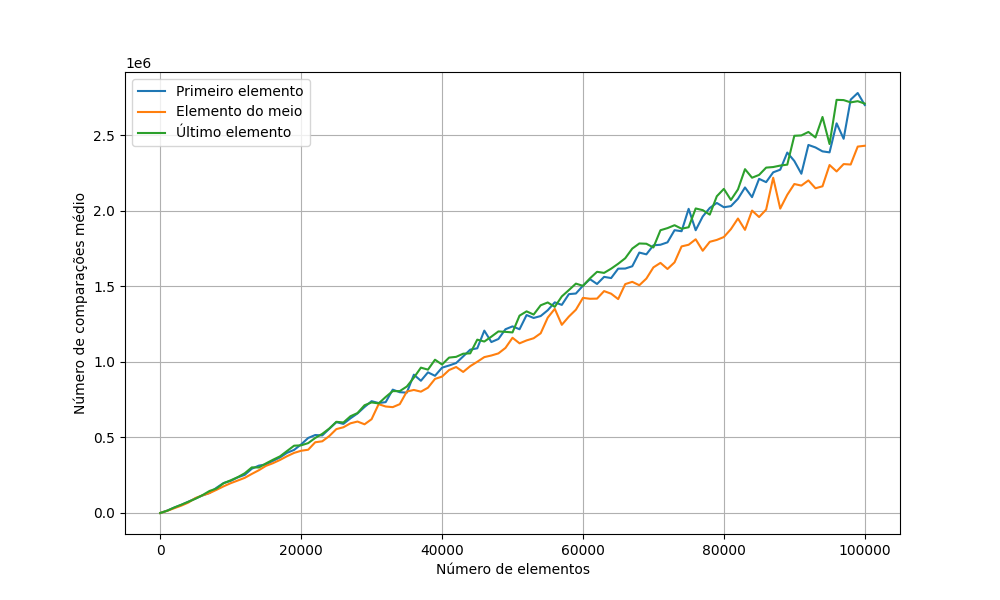
\includegraphics[width=0.85\textwidth]{random.png}
\label{fig:rand}
\end{figure}

Os resultados obtidos destacam a importância de uma escolha adequada de pivô, especialmente em dados ordenados. Em todos os conjuntos testados, a estratégia de escolher o elemento do meio proporcionou o menor número de comparações e, consequentemente, o melhor desempenho do algoritmo.

\section{Conclusão}
Esse estudo ilustra a importância de uma escolha criteriosa para o pivô no Quicksort, demonstrando o impacto significativo que essa decisão pode ter no desempenho do algoritmo. Ao avaliar três tipos de conjuntos de dados, observamos que a escolha do pivô influenciou diretamente o número de comparações necessárias para concluir a ordenação. Especificamente, dados ordenados de forma crescente e decrescente resultaram no pior caso para o algoritmo quando o primeiro ou último elemento eram escolhidos como pivô, mas a seleção do elemento central minimizou as comparações e gerou partições mais equilibradas.

\end{document}
